\chapter{Base de données}

\section{Introduction}
Une base de données est un conteneur permettant de stocker l'intégralité des informations d'une application sur un serveur.
Il existe plusieurs sortes de base de données, mais j'ai décidé de n'en présenter que trois. Ce sont celles utilisées en majorité dans les entreprises.
Il s'agit des bases de données relationnelles (MySQL,PostgreSQL,Oracle, SQLserveur...), des bases de données NoSQL (MongoDB...), et enfin récement de Webstorage.


\section{SGBDR}
Le monde du Système de Gestion de Base de Données Relationnelles est actuellement boulversé par l'arrivée du NoSQL et de nouveaux serveurs comme Node.js.
Mais la plupart des éditeurs de base de données ont compris la nécessité de s'adapter et proposent actuellement une réponse au NoSQL et à Node.js.


\begin{center}
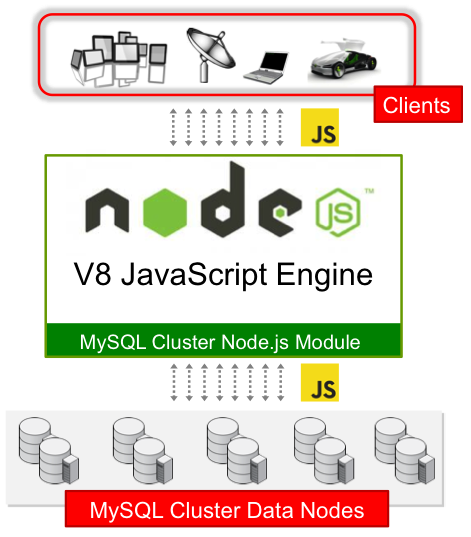
\includegraphics[scale=0.6]{img/mysql_cluster_73_nodejs_figure1.png} 
\label{Graphique technologie mysql cluster}
\end{center}

Afin d'éviter la fuite des développeurs vers des serveurs NoSQL, Oracle par exemple a développer un connecteur NoSQL dans MySQL Cluster 7.3.
Grâce au connecteur NoSQL de MySQL, implanté en tant que module du moteur V8 de Node.js, les utilisateurs peuvent bénéficier de fonctionnalités avancées du SGBDR avec auto-fragmentation pour les applications en plus d’un accès à NoSQL sans transformation en SQL.
La nouvelle API NoSQL Node.js intégrée dans MySQL Cluster offre à Node.js une interface JavaScript asynchrone native qui peut être utilisée à la fois à la requête et à la réception des résultats établis directement à partir de MySQL Cluster, sans transformations en SQL. Cela garantit également une faible latence pour les requêtes simples. Ainsi il est possible en natif d'utiliser uniquement JavaScript pour parler avec MySQL Cluster.

Le fait d'utiliser Node.js permet grace à sa communauté d'accéder à de nombreuses extentions pour utiliser n'importe quelle bases de données relationnelle.
Certaines bases de données incluent également l'accès à la base de données par Webservices ce qui peut éviter l'utilisation d'extentions.

JavaScript est donc capable au travers de Node.js d'accéder à n'importe quelle base de données relationnelle en écrivant ou non du SQL. Cela peut avoir un interêt pour des applications spécifiques ayant besoin de contraintes ACID ou pour éviter aux développeurs et administrateurs de changer leurs habitudes.

Node.js recommande l'utilisation de MongoDB qui est beaucoup plus adapté à sa philosophie que ne le sont les bases de données relationnelles. Ainsi j'ai décidé de parler beaucoup plus en détail de MongoDB et de son intégration parfaite avec Node.js et JavaScript


\section{MongoDB}
\label{ch:mongodb}

\subsection{Présentation}

MongoDB se présente comme une solution évolutive, de haute performance et open source. C’est un type de base de données NoSQL particulier, plus précisément c’est un système de base de données orienté document. MongoDB est écrit en C++.

Pour bien comprendre le concept de base de données orienté document, il faut acquérir une certaine terminologie de base sur MongoDB.

L’écosystème de Node.js possède un excellent support de nombreuses bases de données relationnelles et populaires telles que PostgreSQL et MySQL. Les bases de données relationnelles sont robustes et ont été éprouvées dans le temps, elles sont à même de répondre de manière appropriée aux besoins de nombreuses applications web modernes.

\textbf{Alors pourquoi utiliser MongoDB?}
 
MongoDB a été choisi pour répondre à notre problématique car il propose un ensemble de fonctionnalités caractéristique de ce type de bases de données.

\subsection{Schéma libre}

Un schéma libre signifie qu'il n'y a pas de structure prédéfinie. Une façon simple d’envisager MongoDB est de prendre l’exemple d’un tableau géant d’objets JSON qui est à la fois rapide et puissant dans l’insertion de données et dans ses capacités de recherche.

Parce que toutes les informations de la même entité peuvent être stockées de façon dynamique au sein d’un seul document, rejoindre les opérations n’est plus nécessaire dans ce type de base de données.

Une base de données orientée document est une base de données où plusieurs document d'une même collection peuvent avoir une structure tout à fait différente. Grâce à cette orientation, un certain nombre de champs peuvent être ajouté à un document et ce peut importe la longueur de ces champs. De plus cela est valable même si le document a déjà été créé.

Une opération sur des jointures coûte très cher, ils exigent une cohérence forte et un schéma fixe. Les éviter permet de réduire les coûts et d'augmenter les performances.

\subsection{MongoDB vs SGBDR}

Pour un puriste de la base de données relationnelle, la notion de schéma de base libre peut dérouter. Cependant il y a certains cas d’utillisation où MongoDB offre des avantages sur son homologues traditionnel.

Tout d’abord il est bien adapté pour le développement itératif. Par exemple, imaginons que nous avons une table de personne et que nous souhaitions ajouter une liste de films favoris. Dans une base relationnelle, cela nécessiterait une table de films supplémentaire et une table de jonction pour stocker les relations. En MongoDB cela pourrait se faire en ajoutant simplement une série de films dans la table personne en fonction des besoins. Pour une entreprise en démarrage à l’évolution rapide dont les besoins sont à court terme, et qui dispose d'équipes d'ingénieurs à temps plein, l’agilité de MongoDB peut jouer un rôle important.
MongoDB est également approprié pour les données non structurées. Dans le monde de la finance qui dispose de milliers de type de données différentes, utiliser une base de données relationnelle poserait un certain nombre de défis mais en utilisant MongoDB c’est aussi simple que représenter les données en JSON et les insérer dans la base de données.
En outre MongoDB a été conçu dès le départ pour le big data, qui est soutenu par un mécanisme connu sous le nom de fragmentation permettant d'accélérer la recherche.

D’autre cas d’utilisation de MongoDB sont discutés en détail sur le site officiel.

\subsection{JavaScript}

Les demandes faites à MongoDB sont écrites en JavaScript, ce qui est parfait pour une application 100\% JavaScript. En outre, ces demandes utilisent une requête de style SGBDR qui réduit l’écart et permet aux développeurs habitués à un langage traditionnelle de requête structurées de s'adapter.

\subsection{Types de données}

MongoDB utilise BSON pour le stockage des données et comme format de transmission réseau. BSON signifie “Binary JSON”, il s'agit d'une sérialisation binaire codé en JSON-like.
Selon le bsonspec.org, il a été conçu pour être léger, transversal et efficace.

Son principal avantage sur XML et JSON est l’efficacité en terme d’espace et de temps de traitement.

Les documents BSON peuvent être utilisés pour stocker plusieurs types de données comme “string, integer, boolean, double, null, array, objet, date, données binaires, expression régulière et code source".

\subsection{JSON Document-Oriented}

MongoDB utilise le format JSON parsé comme structure de données. Les données envoyées à MongoDB peuvent être stockées immédiatement et sans aucun prétraitement. L’approche clé/valeur d’autres bases de données NoSQL comme Redis n’est pas convenable en cas de stockage de valeur plus important qu’une seule valeur.

\subsection{Temps-réel}

MongoDB est très bon pour insérer en temps réel des données et garder un support de transaction extrêmement simple.
Il est rapidement devenu la base de données de facto pour Node.js. Jason Hoffman, fondateur de Joyent, a donné une présentation sur Node.js et MongoDB comme étant LA pile moderne pour le Web temps réel en remplacement de la couche LAMP traditionnelle (Linux, Apache, MySQL, PHP).

\subsection{Fonctionnalités avancées}

MongoDB possède un ensemble de fonctionnalités avancées telles que l’index complet, la réplication, la fragmentation et le map/reduce.

\subsection{Connecteur NodeJS}

MongoDB a un pilote source natif et ouvert écrit par Christian Amor Kvalheim appelé node-mongodb-native.
https://github.com/christkv/node-mongodb-native

\subsection{Conclusion}

MongoDB et plus généralement le mouvement NoSQL, offre une nouvelle approche sur l’utilisation des bases de données. MongoDB a remplacé le SQL par du JavaScript ce qui aurait pu être un facteur inquiétant à première vue, mais il s'est finalement trouvé rapide et facile à apprendre et très flexible.

Un grand merci à son interpréteur JavaScript qui permet de commencer à pratiquer MongoDB très rapidement. En fait, vous pouvez même commencer sans l’installer en utilisant le site try.mongodb.org qui propose un tutoriel interactif pour apprendre MongoDB.

Comme le nombre important et croissant de pilotes est disponible (Java, Scala, C\#, Erlang, C, C++, etc), MongoDB évolue rapidement et à été mis en open source en 2009 par 10gen l’éditeur.

\section{Web Storage}

\subsection{Présentation}

Lorsque les développeurs Web pensent à stocker des données utilisateurs, leur premier réflexe consiste à télécharger ces données sur le serveur. HTML5 vient révolutionner tout cela, puisqu'il existe désormais plusieurs technologies permettant aux applications d'enregistrer des données sur un appareil client. Ces données peuvent également être synchronisées avec le serveur ou ne demeurer que sur le client : la décision revient au développeur.

Le stockage côté client est avantageux pour plusieurs raisons. Tout d'abord, il vous permet de faire fonctionner l'application lorsque l'utilisateur est hors connexion, et éventuellement, de synchroniser les données une fois la connexion au réseau rétablie. Ensuite, il vous permet de booster vos performances. En effet, vous avez la possibilité d'afficher un important corpus de données dès que l'utilisateur clique sur votre site, au lieu de devoir attendre qu'il soit de nouveau téléchargé. Enfin, il s'agit d'un modèle de programmation plus simple, pour lequel aucune structure de serveur n'est nécessaire.


Le principe est vraiment très simple : c’est un stockage sous la forme clé / valeur. Il y en a deux différents :
\begin{list}{•}{}
  \item
  stockage uniquement pour la durée de la session (et uniquement pour cette instance du site, un autre onglet sur la même page n’est pas affecté) ;
    
  \item
  stockage permanent.

\end{list}
 Pour chacun de ces stockages, on a un objet manipulable, respectivement sessionStorage et localStorage. Les deux objets exposent la même API.
 
 Comme il s'agit d'une API, JavaScript peut l'utiliser. Ainsi il est facile de créer des applications stockant des données sur le client et n'utilisant pas de base de données. On peut également mélanger webstorage avec un serveur de base de données. Afin de permettre un mode offline d'une application web.

\section{Conclusion}

Actuellement les bases de données sont en évolution car de nouvelles tendances arrivent et bousculent le marché du stockage des données.
JavaScript est actuellement capable, au travers d'API dédiées ou de Node.js, de se connecter à n'importe quelle base de données. Que ce soit une base de données relationnelle, une base de données NoSQL, une base de données NewSQL et meme aucun serveur avec l'api Web Storage. Le fait que la plupart des bases de données NoSQL utilisent JSON en font une solution très pertinente pour stocker rapidement et simplement des données sans nécessiter un travail complexe. C'est pourquoi à mon avis il est beaucoup plus pertinent d'utiliser une solution de type NoSQL comme MongoDB plutôt que le traditionnel MySQL ou un autre SGBDR. Mais comme dans ma partie Client léger, il est pour l'instant trop tot pour se prononcer. Le choix reste pour l'instant aux développeurs car aucune solution ne sort actuellement du lot. La bataille se joue actuellement pour imposer le standard de la base de données Node.js. MongoDB se démarque du lot en étant disponible en natif dans Node.js

